\documentclass[9pt]{beamer}
\usetheme{test}






\logo{
\includegraphics[height=0.5cm]{logo_beamer.PNG}}
\title{Outils d'apprentissage automatique.}

\subtitle{Cours 1: Apprentissage automatique avec scikit-learn.}

\author[Djeachandrane, Mellouk, Zeghlache] % (optional, for multiple authors)
{Pr.~A.~Mellouk\inst{1} \and A.~Djeachandrane\inst{1} \and R.~Y.~Zeghlache\inst{1}}

\institute[EPISEN-ITS] % (optional)
{
  \inst{1}%
  EPISEN, LISSI, UPEC, Universite Paris-Est, 94400 Vitry sur Seine, France\\}


\centering
\date{28 Octobre 2020}
\begin{document}
\maketitle
\begin{frame}{Sommaire}
\begin{itemize}
\item Objectif de scikit-learn.
\item Python et son éco-système pour l'apprentissage automatique.
\item Les types d'apprentissages.
\item Que peut-on faire avec scikit-learn?
\item Fonctionnement de la librairie.
\item Quelques Ressources.


\end{itemize}
\end{frame}



\begin{frame}{Objectif de scikit-learn.}
\framesubtitle{Rester le plus simple possible..}
    \begin{block}{Pas besoin de besoin de pré requis en ML.
}    Tout le monde peut utiliser la lib, sans connaître un seul algorithme ! Seulement la programmation python est requise.
    \end{block}
    
    
    \begin{block}{Pas de domaine d'application spécifique.}
    On peut utiliser la lib pour tous types de problématiques envisageable: Santé, économie, Marketing ,Télecom, ect..
    \end{block}
    \begin{block}{Hérite de la simplicité et de la flexibilité de python.}
    Permet d'avoir un code lisible et simple tout en gardant un haut niveau d'abstraction.
    \end{block}
\end{frame}




\begin{frame}{Python et son éco-système pour l'apprentissage automatique.}
\framesubtitle{L'équipe de choc: Numpy, Matplotlib, Pandas, Scipy}


\includegraphics[height=1.5cm]{ecosystem.jpg}
   \begin{itemize}
       \item Numpy: Module pour manipuler les Arrays en python.
       \item Matplotlib: Module de visualisation en python.
       \item Scipy: Module de calcule scientifique et mathématique.
       \item Pandas: Module pour manipuler les dataframes, lire et créer des tabulars.
\end{itemize}
\end{frame}


\begin{frame}{Les types d'apprentissages supporté par scikit-learn.}
\begin{itemize}
\begin{block}{Apprentissage supervisé:}
Nous avons des données en entrée (Variables de décisions ou Features) et le résultat attendu (\'Etiquettes ou Labels). Il nous permet de faire des prédictions basées sur un modèle qui est obtenu à partir de données d’historique et d'un ’algorithme choisi.
\end{block}
\begin{block}{Apprentissage non supervisé:}
Avec cet apprentissage, nous avons toujours des features, mais plus de label, ici nous n’essayons pas de prédire quoi que ce soit. À partir des données historiques que nous avons, nous essayons de voir ce que nous pouvons apprendre des données.
\end{block}
\begin{block}{Apprentissage faiblement supervisé:}

L'apprentissage semi-supervisé est une classe de techniques d'apprentissage automatique qui utilise un ensemble de données étiquetées et non étiquetées.
\end{block}

\end{itemize}

\end{frame}


\begin{frame}{Ce qu'il est possible de faire avec scikit-learn.}
 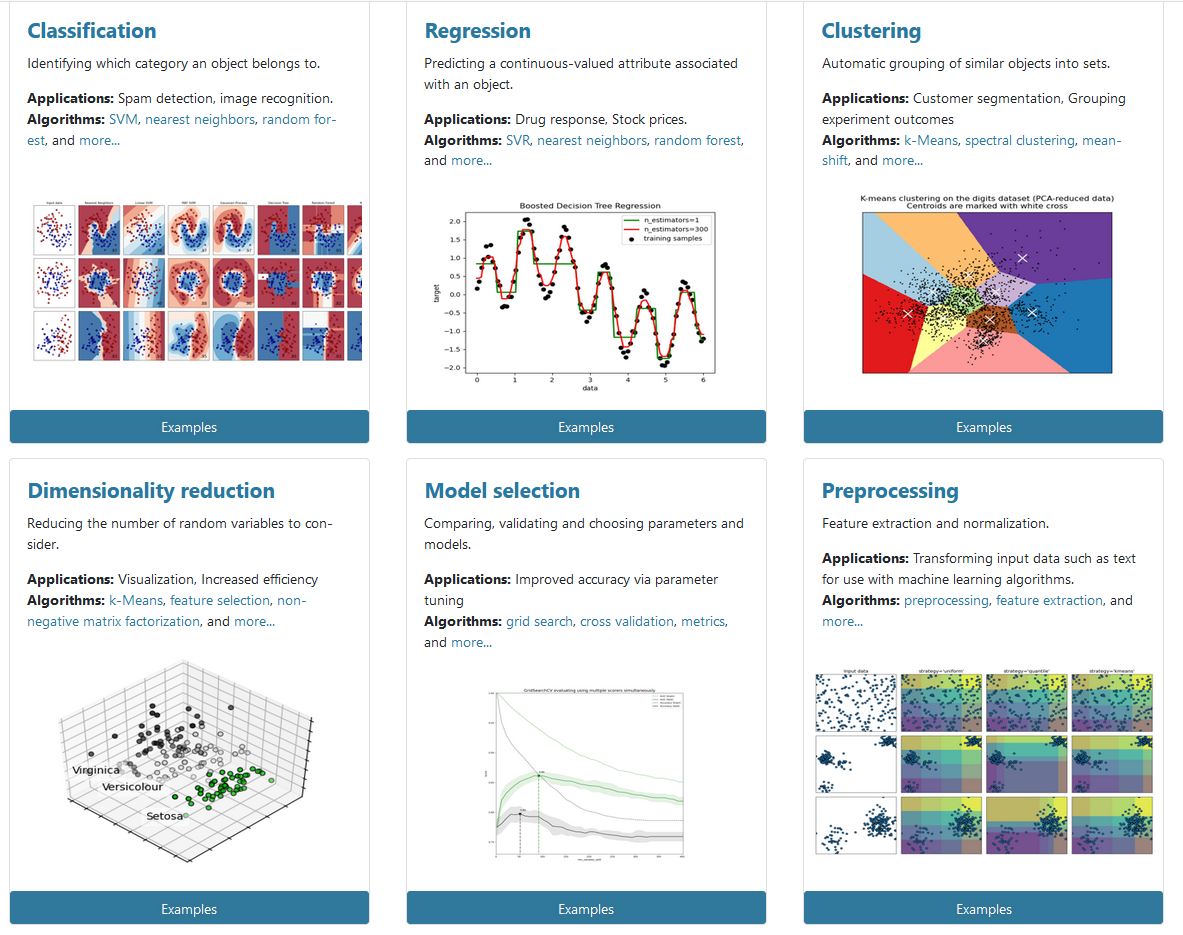
\includegraphics[height=6.8cm]{scikitlearnoverview.PNG}
\centering   
\end{frame}



\begin{frame}{Processus simple d'apprentissage avec scikit-learn.}
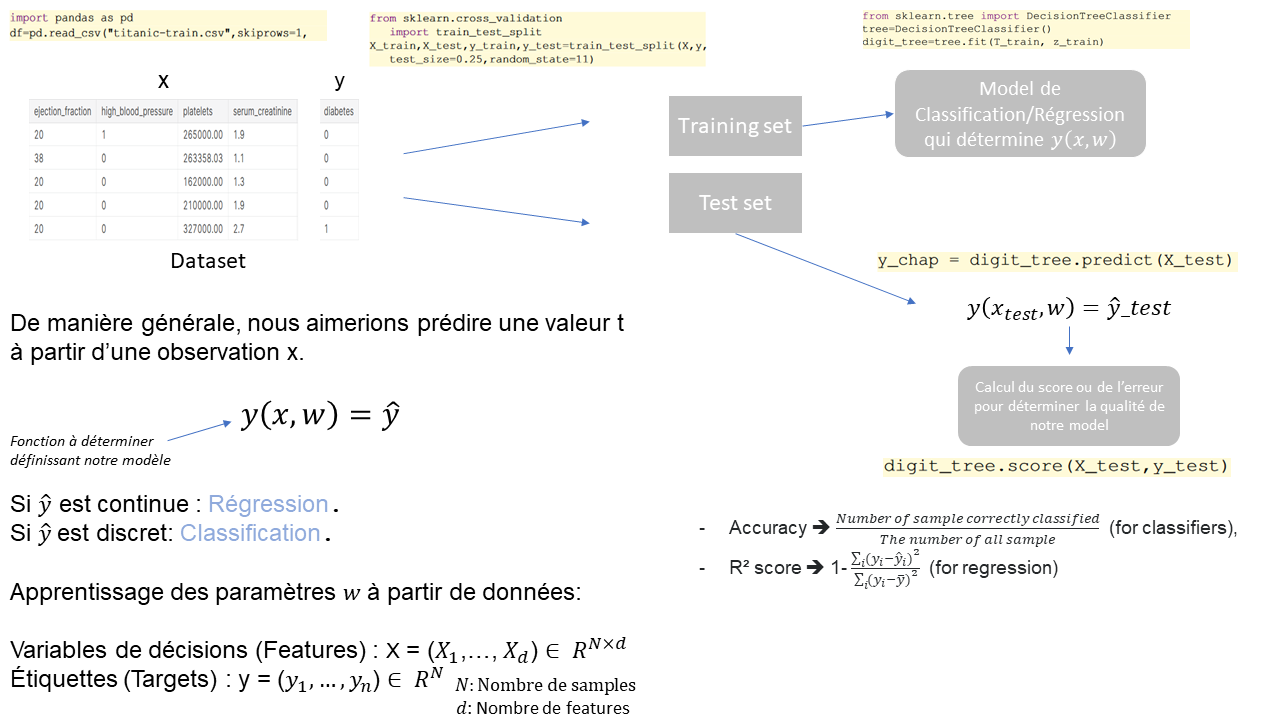
\includegraphics[height=6.8cm]{Diapositive1.PNG}
\centering   
\end{frame}


\begin{frame}{Workflow classique d'un projet d'apprentissage.}
\begin{block}{Les \'Etapes sont les suivantes:}
\begin{itemize}
    \item \textbf{1.Application de pré-traitements sur notre dataset: Normalisation, conversion, ect..}
    \item \textbf{2.Sélection des "meilleurs" features.}
    \item \textbf{3.Split le dataset en Train/Validation/Test set et appliquer une validation croisée.}
    \item \textbf{4.Sélection du "meilleur" modèle et des ses hyper-paramètres.}
    \item \textbf{5.Tester le modèle sur un dataset qu'il n'a pas vu ni en entraînement ni en validation.}
    \item \textbf{6.Recommencer jusqu'à atteindre l'objectif de précision définie :).}
\end{itemize}

\end{block}
    
\end{frame}




\begin{frame}{Pré-traitement avec scikit-learn et pandas}
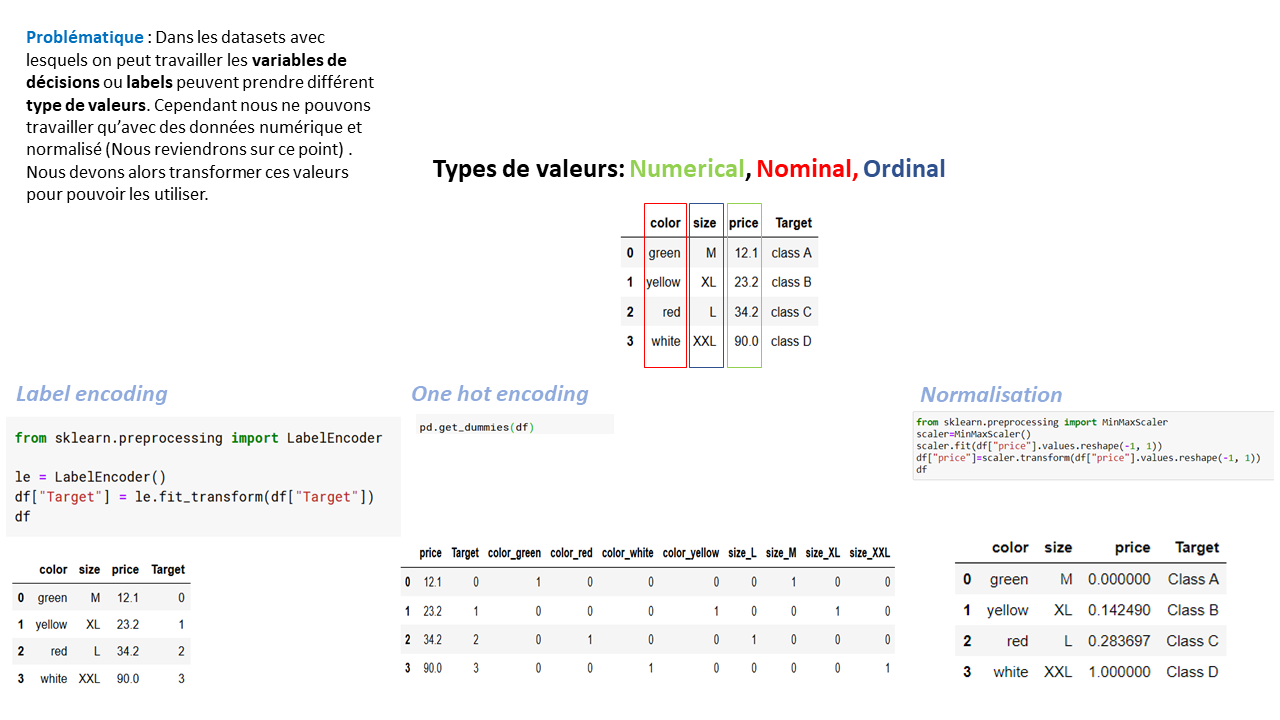
\includegraphics[height=6.3cm]{Diapositive2.PNG}
\end{frame}

\begin{frame}{Partitionnage et validation croisé}
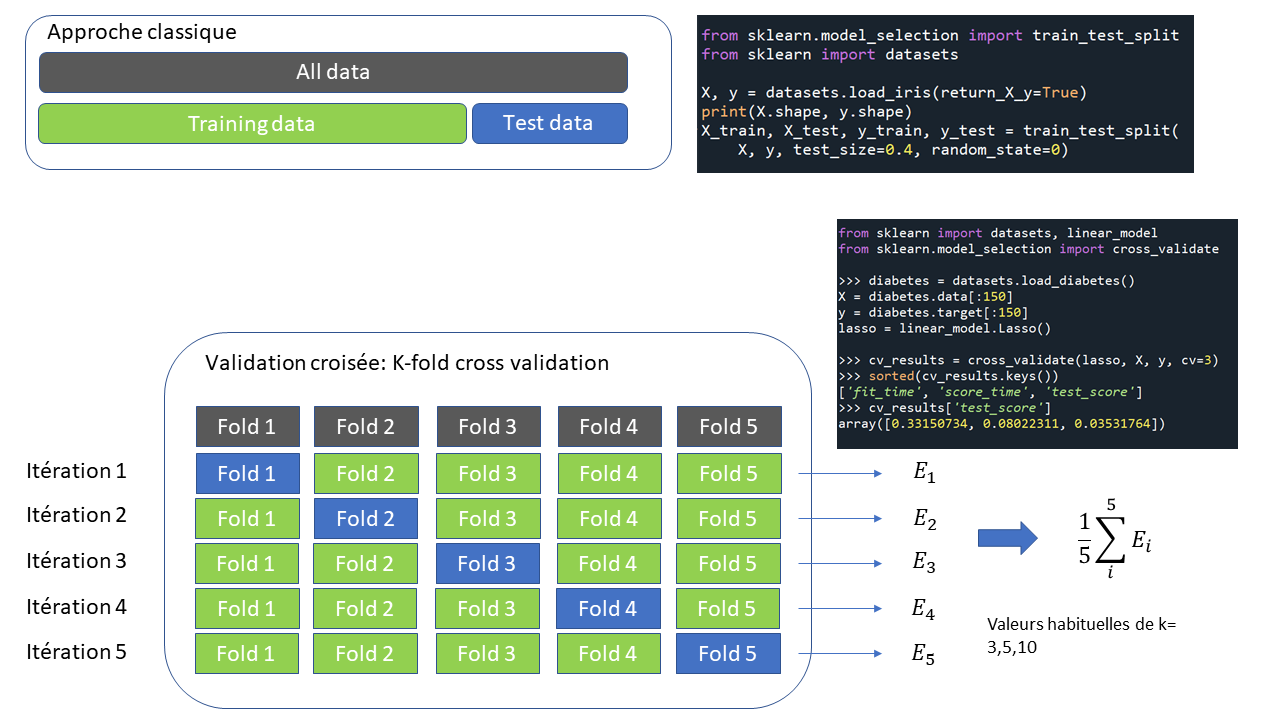
\includegraphics[height=6.3cm]{Diapositive3.PNG}
\end{frame}


\begin{frame}{Sélection des features (Pour plus tard)}
Nous verrons cela en detail plus tard.
\end{frame}

\begin{frame}{L'objet Estimator}
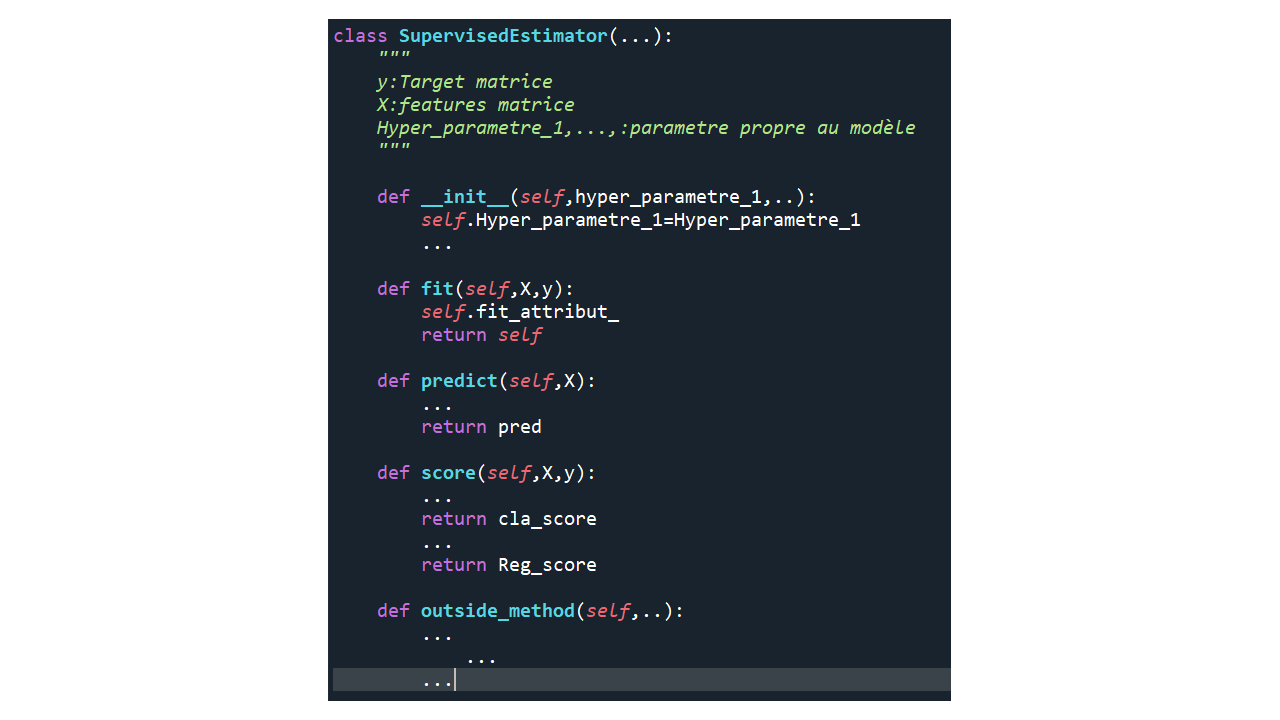
\includegraphics[height=6.3cm]{Diapositive4.PNG}
\end{frame}

\begin{frame}{API centrale de scikit learn: Estimator}
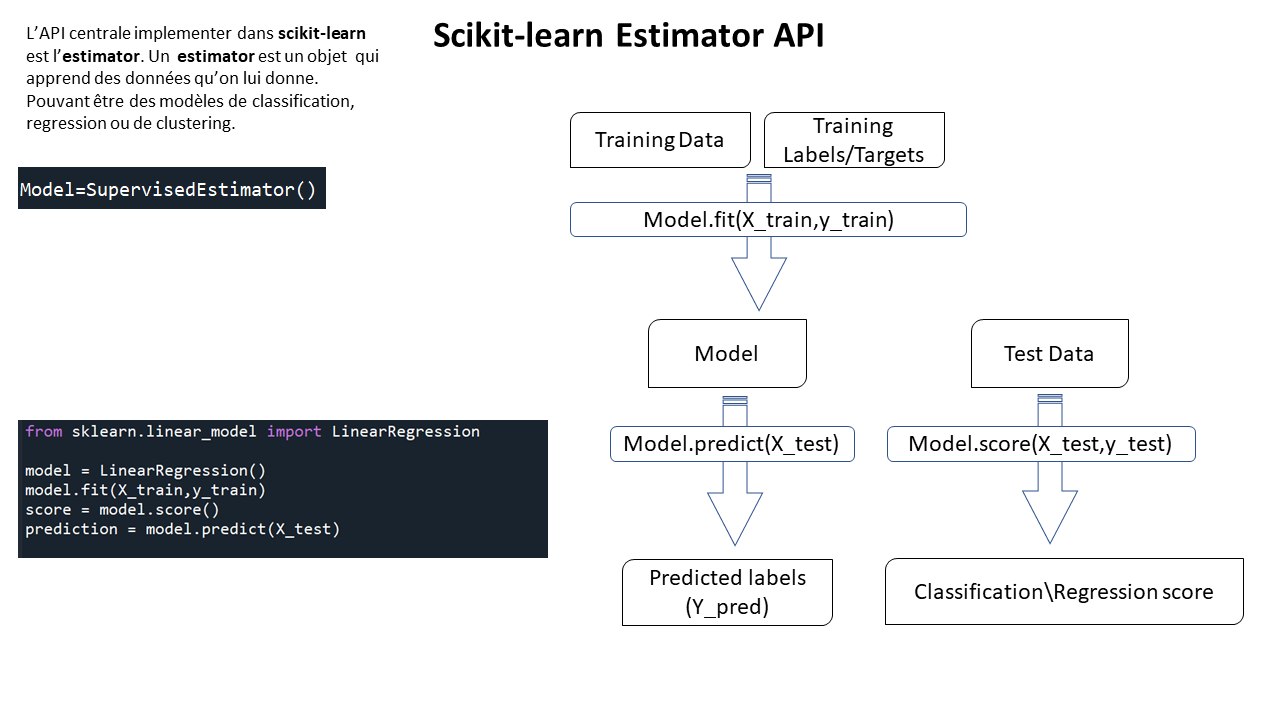
\includegraphics[height=6.3cm]{Diapositive5.PNG}
\end{frame}


\begin{frame}{L'objet transformer}
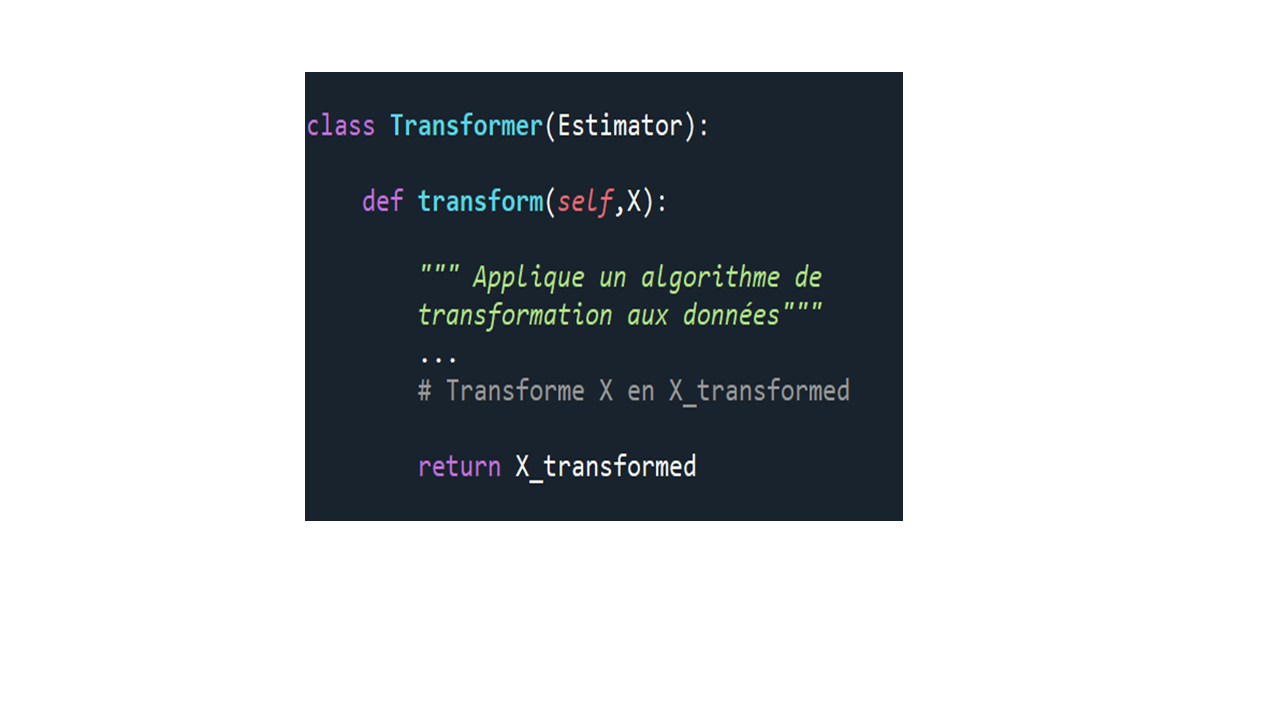
\includegraphics[height=6.3cm]{Diapositive6.PNG}
\end{frame}

\begin{frame}{L'API transformer}
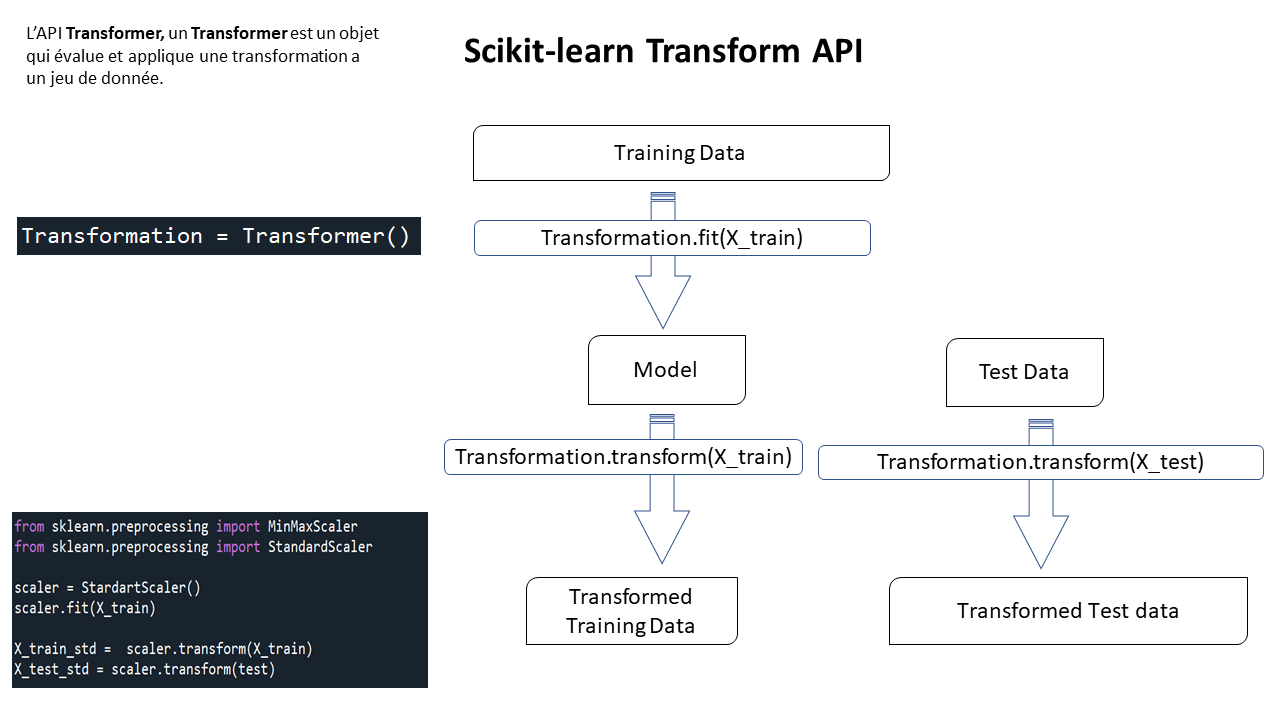
\includegraphics[height=6.3cm]{Diapositive7.PNG}
\end{frame}


\begin{frame}{L'API Pipeline}
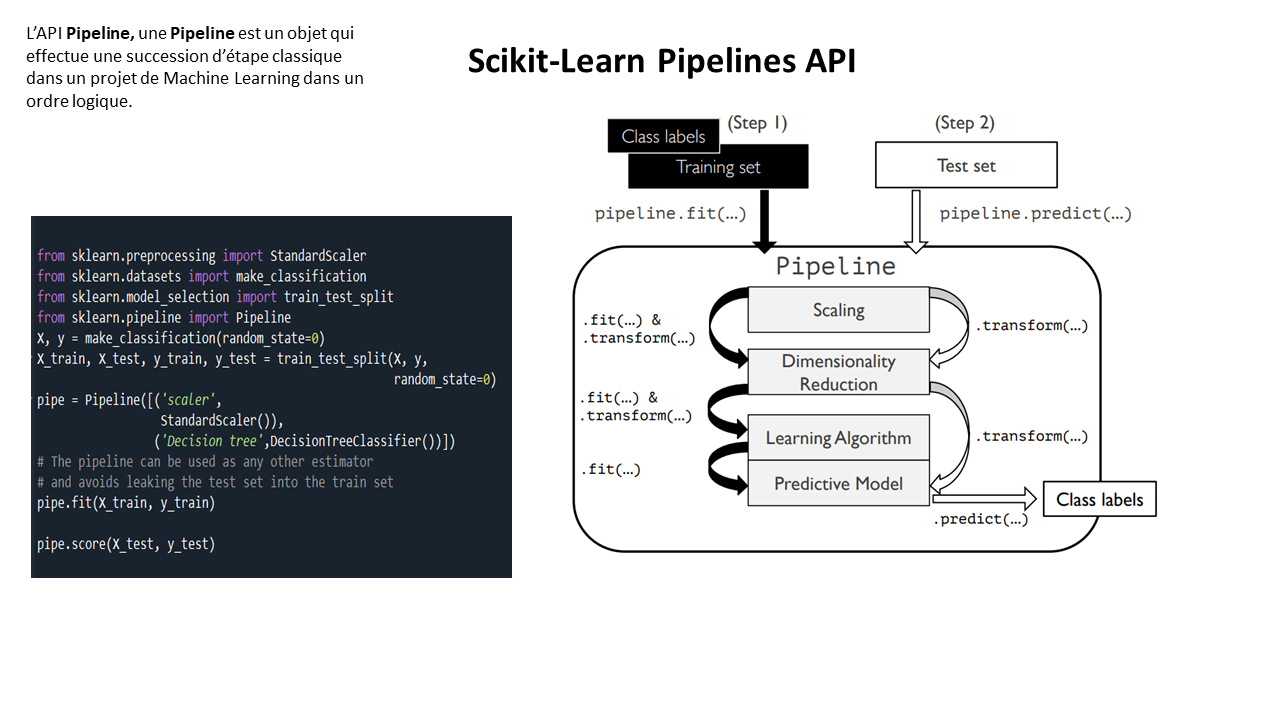
\includegraphics[height=6.3cm]{Diapositive8.PNG}
\end{frame}


\begin{frame}{API Model selection}
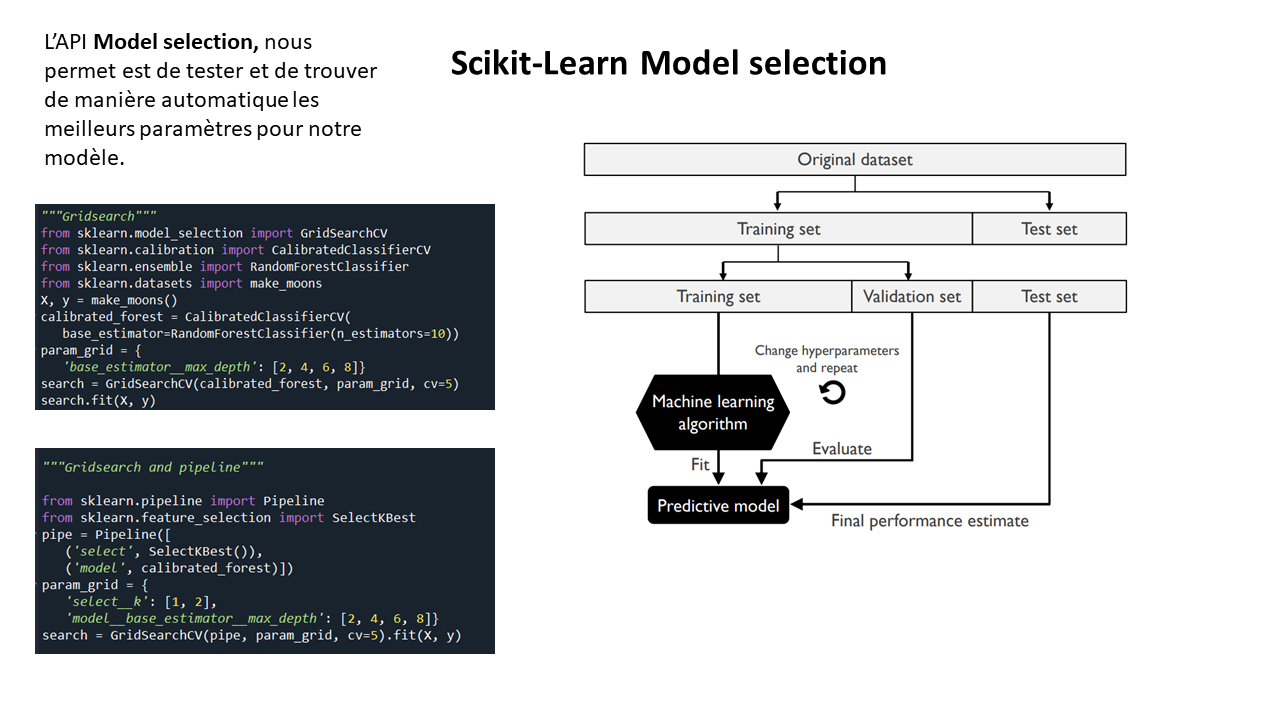
\includegraphics[height=6.3cm]{Diapositive9.PNG}
\end{frame}



\begin{frame}{Quelques ressources}
\begin{itemize}
    \item https://scikit-learn.org/stable/ (site de la librairie, à étudier absolument)
    \item Learning scikit-learn: Machine Learning in Python (Anglais) 2013 de Raúl Garreta (Auteur), Guillermo Moncecchi (Auteur)
    \item  Machine Learning avec Scikit-Learn - 2e éd. - Mise en oeuvre et cas concrets: Mise en oeuvre et cas concrets (Français) de Aurélien Géron (Auteur)
    \item scikit-learn Cookbook - Second Edition: Over 80 recipes for machine learning in Python with scikit-learn (Anglais) Broché – 16 novembre 2017 de Julian Avila (Auteur)
    \item https://www.kaggle.com/search (Temple de la science des données)
    \item https://www.coursera.org/ (Un grand nombre de projet guidé gratuit sur scikit-learn)


\end{itemize}
\end{frame}


\begin{frame}
\huge{\centerline{Fin. Merci pour votre attention !}}
\end{frame}

\end{document}
